\documentclass[a6paper,10pt]{ctexbook}
\usepackage[utf8]{inputenc}
\usepackage{xcolor,pagecolor}
\usepackage[margin=1.25cm, paperwidth=105mm, paperheight=163mm]{geometry}
\usepackage{xeCJK,fontspec,setspace,endnotes,graphicx,tikz}
\usepackage[defaultlines=2,all]{nowidow}
\usepackage{enumitem}
\setCJKmainfont{STHeiti}
\setCJKsansfont{LXGW WenKai TC}
\setmainfont{Noto Serif}
\setsansfont{Noto Sans}
\setlength{\parindent}{2em}
\setlength{\parskip}{6pt}
\pagecolor{white}
\setlist{nosep}
\let\footnote=\endnote

\newcommand{\remark}[1]{\vspace*{2pt} \textsf{#1}\vspace*{2pt}}
\renewcommand{\notesname}{註解}

\title{\textbf{第十六世噶瑪巴觀想法} \\[6pt] \large 金剛乘佛法常用之上師相應修行法}
\date{}
\pagestyle{empty}
\begin{document}
\color{black}
\maketitle

\vspace*{\fill}
{
  \small\sffamily\noindent\copyright{} 2024 台灣金剛乘佛法\\ (Diamond Way Buddhism Taiwan)

\noindent 2024年7月出版於台灣高雄市

\noindent https://diamondway-buddhism.org\\
https://diamondway.tw\\
contact@diamondway.tw
}

\cleardoublepage
\vspace*{3ex}
親愛的朋友們,

此版本第十六世噶瑪巴觀想法出於二零一零年冬。在六十年代後期,第十六世噶瑪巴朗炯瑞沛多傑,讓漢娜和我持有了這個實用而全面的覺悟工具。遵照他的願望——讓這個觀想法一直有生氣地、合乎時代地對應西方人的心,我們多次改變了修行重點。此版本重點在於,把修法中得到的純淨觀點積極地持續到我們的日常生活中。

每天早上皈依後,我們可以在當天無需形式地隨時讓上師出現在前方,接受他的加持。我不知道還有甚麽比這更有效的修煉方法。那麽,讓我們練習和享受吧!

\noindent%
\begin{tikzpicture}[blend group=multiply]%
  \node{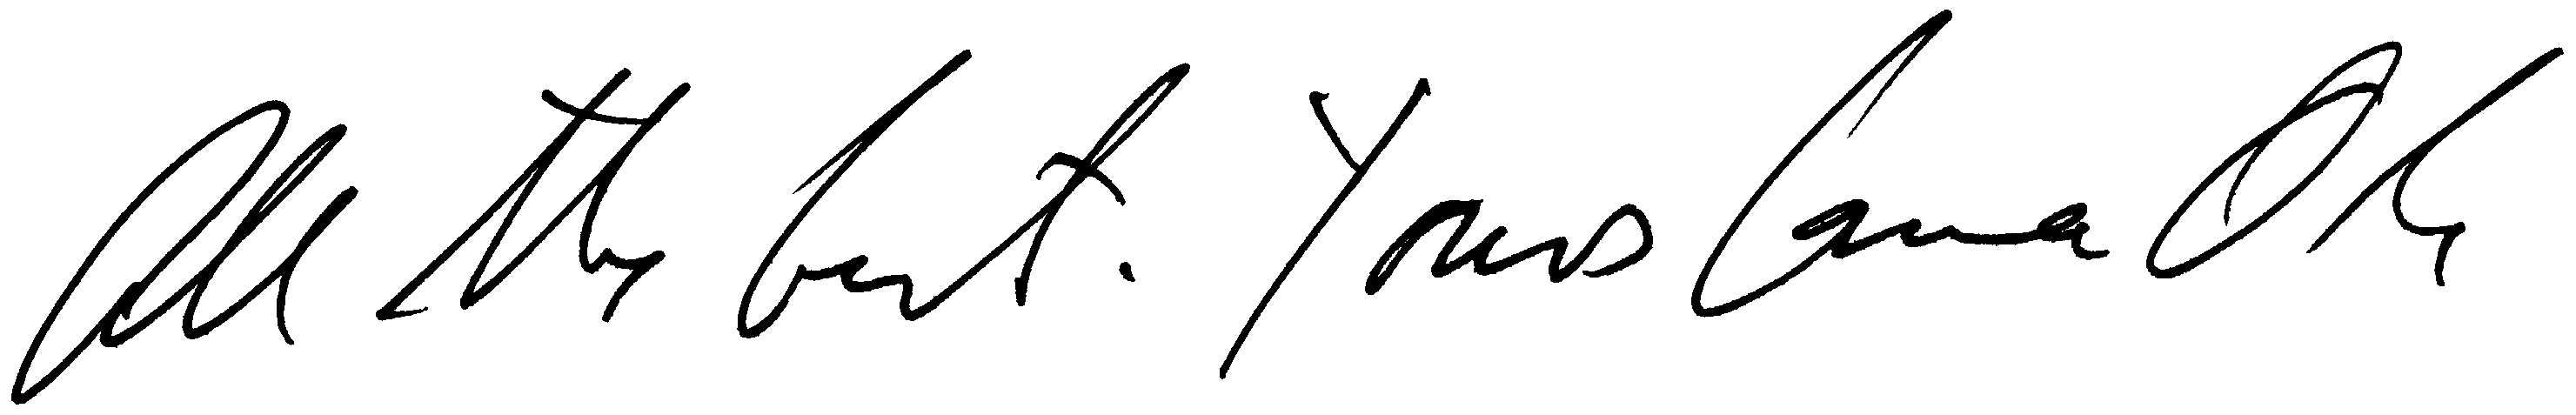
\includegraphics[width=0.9\textwidth]{signature_en.png}};
\end{tikzpicture}

祝福大家一切都好!

你們的歐雷喇嘛

\cleardoublepage
\section*{第十六世噶瑪巴觀想法}

我們感受著呼吸的無形氣流自鼻尖進進出出,讓思想和聲音來來去去,不加以評判。
\vspace{-3ex}

\section*{四個基本觀念}

然後專注於四個基本觀念,使心轉向解脫和覺悟:

我們慶幸此生能有這份珍貴的機會,得以運用佛陀的教法來利益無量眾生。只有少數的人能夠與金剛乘教法相遇,其中有能力加以運用的人更是少之又少。

我們提醒自己,萬事萬物都會改變\footnote{因緣和合之物皆流轉無常},只有心那無限及清晰的『空』是永恆的。沒有人知道,使我們能夠認識這樣真理\footnote{實相}的條件還會存在多久。

我們明白因果,因此知道發生的事由我們自己決定。過去的思想、語言與行為導致我們今天的狀況,同時我們還為未來不斷種下新的因子。

最後我們明白,為甚麽要在心上下功夫:覺悟意味著永恆的最高快樂,而只要我們自己還陷於迷惑和煩惱中,我們就不能利益他人。

\section*{皈依及覺悟的心願}

現在我們向那些能教導我們的,敞開自己的心。為了帶領眾生通往覺悟,我們

\begin{itemize}
\item
  皈依佛——心的完全展現;
\item
  皈依教法——引領我們到彼岸;
\item
  皈依菩薩——佛道上的朋友;
\item
  特別是皈依上師,在此為第十六世噶瑪巴。上師集加持、修法和護持於一身,是我們快速發展之所需。\footnote{此段即通稱之三皈依或四皈依:皈依佛、法、僧、金剛上師。注意此處之四皈依是觀想內容,並不代表也不強迫成為金剛乘佛教的佛門子弟}\footnote{在巴利文中,三皈依(Tisarana)是由三(ti)與庇護所(sarana)所組成,意為由佛、法、僧構成的一個三重庇護所}
\end{itemize}

\newpage
\section*{呈現階段}
\vspace{-6ex}

受到條件約束的世界,在此消融成為『空』。\footnote{有為法消於空}

\remark{我們沈浸在『空』的寬廣中。}

在我們前方,聚起了金色的、透明的第十六世噶瑪巴的形象——
一個閃爍著光芒的光能場。

噶瑪巴頭頂著黑寶冠,這頂寶冠能喚醒我們心底最深沉的覺知。噶瑪巴的面孔金色溫和,他注視著我們,也瞭解我們,並祝福我們。

噶瑪巴的手臂交叉於胸前,雙手各持金剛杵和金剛鈴,意味著慈悲與智慧不可分。噶瑪巴持蓮花座\footnote{結跏趺坐},彩虹光圍繞。

噶瑪巴集空性和喜悅於一身,行萬佛之事業。噶瑪巴就在這裏,不論我們是否能清晰感受到他的形象。我們深深祈願,為了利益眾生,自己能實現他那樣的覺悟品質。

噶瑪巴瞭解我們的願望,他微笑著,穿越空間,離我們越來越近。現在噶瑪巴停留在我們的前方,保持著舒適的距離。

「敬愛的上師——所有佛的本質,請顯示給我們力量,除去眾生及我們自己的無知和障礙,願我們認識心那永恆的光。」

\setlength{\parskip}{3pt}

\section*{加持階段——身業}

從噶瑪巴的雙眉間射出一道強烈而清澈的光進入我們的雙眉間,充盈我們的頭部。

這道光將去除大腦、神經和感官裏的一切煩惱印跡,所有有害行為的業因都消失了,我們的身體放鬆下來。我們的身體成為了保護和幫助他人的意識工具。

我們沉浸在這道透明的光裏,時間長短如己所願,同時感受著咒音——嗡(OM)。

\remark{持住於此光和震音之中。}

\section*{加持階段——語業}

從噶瑪巴的喉嚨射出一道強烈的紅光進入我們的口和喉嚨。

這道透明的光融化了我們語言上的障礙,由粗口和妄語所留下的惡業消失了。我們將有意識地運用語言,它現在充滿慈悲和智慧,成為了幫助眾生的強大工具。

與紅色光一起,我們感受著咒音——啊(AH)。

\remark{持住於此光和震音之中。}

\section*{加持階段——意業}

從噶瑪巴透明的身體中央,由心中射出一道強烈的藍光填滿我們胸中。

現在心中所有傷害性的東西都消失了,煩惱和固執的成見去除了,我們的心回歸了自在的歡喜\footnote{無作意歡喜},空性與快樂不可分。

與藍色光一起,我們體會著咒音——吽(HUNG)。

\remark{持住於此光和震音之中。}

\section*{大手印加持\footnote{Mahamudra,英文直譯Great Seal, Great Imprint,中文常譯為大手印。大手印的直接意思是:『空』及智慧不可分割這樣的事實,烙印在所有的現象中。在此文簡短稱呼為萬相合一的境界}}
三道光同時射入我們:清澈的光進入額頭、紅色的光進入喉頭、藍色的光進入心臟。

我們毫不費力地持住於萬相合一之噶瑪巴境界中。

\remark{同時持住於這三道光中。}

現在我們運用咒語KARMAPA CHENNO「噶瑪巴虔喏」,意思是「願我們能行萬佛之事業」。

\begin{center}\large\bfseries
噶瑪巴虔諾

KARMAPA CHENNO
\end{center}

\section*{完滿和見地}

在我們前方,金色的噶瑪巴和他的黑寶冠溶入彩虹光中。

這道光射入我們,遍佈空間,所有形式都消失了。

現在只有覺知,無中心也無邊界。

\remark{持住於心性中。}

所有顯現於心的,都是『空』自在的遊戲。

\remark{持住於心性中。}

我們四周顯現出這個世界和所有世界,完美而純淨。每個微粒子都因快樂而震動,因愛而聚集。一切都是那麽新鮮有意義,充滿著無邊無際的可能。

遠近眾生皆示現為女性或男性的佛,不論他們自己是否知道。

聲音就是咒語,思想就是智慧,因為它們能夠顯現。

我們感覺到自己的身體在空間中聚起,充滿了力量和快樂。但與過去有了本質區別:過去,我們『是』這個身體,由於衰老、病痛、死亡和失去而易受傷害。現在我們『持有』這個身體,身體和語言是利益他人的意識工具。

我們現在知道了,真正的我們,是永恆的覺知,無中心也無邊界,遊戲自在地顯現一切。

\section*{迴向}

我們決定,在任何生活情況中都保持這個純淨的觀點,並祈願,剛才產生的好印象,將擴展至無限,希望能帶給眾生那唯一持久的幸福——心性的認識。
\newpage
\theendnotes

\end{document}

